\section{Single-link Manipulator Model}
The modelling of the single-link manipulator has been carried out using
\href{https://www.mathworks.com/products/simulink.html}{MATLAB Simulink}, as
well as for the rest of the models found in this report.

The data that describes the single-link manipulator has been summarized in
\autoref{table:model-data} It has been modelled in two different ways, which
have been compared.

\begin{table}
\centering
\begin{tabular}{c | c | c}
    Description & Variable & Name \\
    \hline\hline
    Moment of inertia of the rotor & $J_m$ & $6.1e^{-4} kg m^2$ \\
    \hline
    Electromotive force constant & $K_b$ & $0.105 \frac{V}{rad/s}$ \\
    \hline
    Motor torque constant & $K_m$ & $0.105 \frac{N m}{A}$ \\
    \hline
    Armature inductance & $L$ & $0.9e^{-3} H$ \\
    \hline
    Armature resistance & $R$ & $0.76 \Omega$ \\
    \hline
    Motor viscous friction constant & $B_m$ & $4e^{-4} \frac{N m}{rad/s}$ \\
    \hline
    Effective damping & $B$ & $1.49e^{-2} \frac{N m}{rad/s}$ \\
    \hline
    Gear ratio & $r$ & $156$ \\
    \hline
    Lower saturation input signal limit & $Vmin$ & $-35 V$ \\
    \hline
    Upper saturation input signal limit & $Vmax$ & $35 V$ \\
    \hline
\end{tabular}
\\ [1ex]
\caption{Single-link manipulator data}
\label{table:model-data}
\end{table}

\subsection{Accurate model (Task 1)}
\label{subsec:accurate-model}
An accurate model of the single-link manipulator is shown in
\autoref{fig:accurateManipulatorModel}, the specifics of how this model is
derived can be found in \citetitle{SingleLink} \cite{SingleLink}.

\begin{figure}
    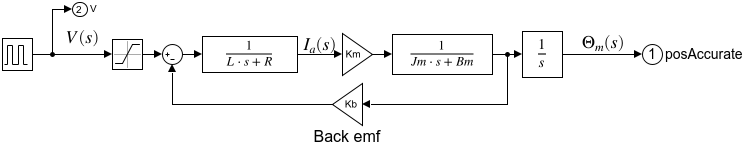
\includegraphics[width=\textwidth]{accurateManipulatorModel.slx.png}
    \caption{Accurate manipulator Simulink model}
    \label{fig:accurateManipulatorModel}
\end{figure}

\subsection{Simplified model (Task 2)}
\label{subsec:simplified-model}
After some manipulation of the \nameref{subsec:accurate-model} and neglecting
the electrical time constant $\frac{L}{R}<<\frac{J_m}{B_m}$ \cite{SingleLink}
one can obtain the simplified model of the single-link manipulator shown in
\autoref{fig:simplifiedManipulatorModel}.

\begin{figure}
    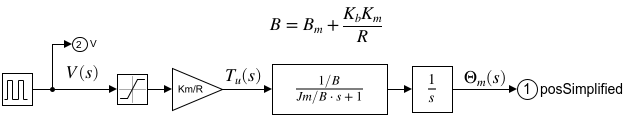
\includegraphics[width=\textwidth]{simplifiedManipulatorModel.slx.png}
    \caption{Simplified manipulator Simulink model}
    \label{fig:simplifiedManipulatorModel}
\end{figure}

\subsection{Comparison}
These two models have been compared by means of a simulation carried out in
Simulink. Which shows the system response to a pulse input.
\autoref{fig:modelAccurateVsSimplified} shows the results of this comparison.
It is easy to appreciate that the simplified model is sufficiently accurate to
be used as the single-link manipulator model. Its computational efficiency and
simplicity make it a better choice than the accurate model for the rest of the
report simulations.

\begin{figure}
    \centering
    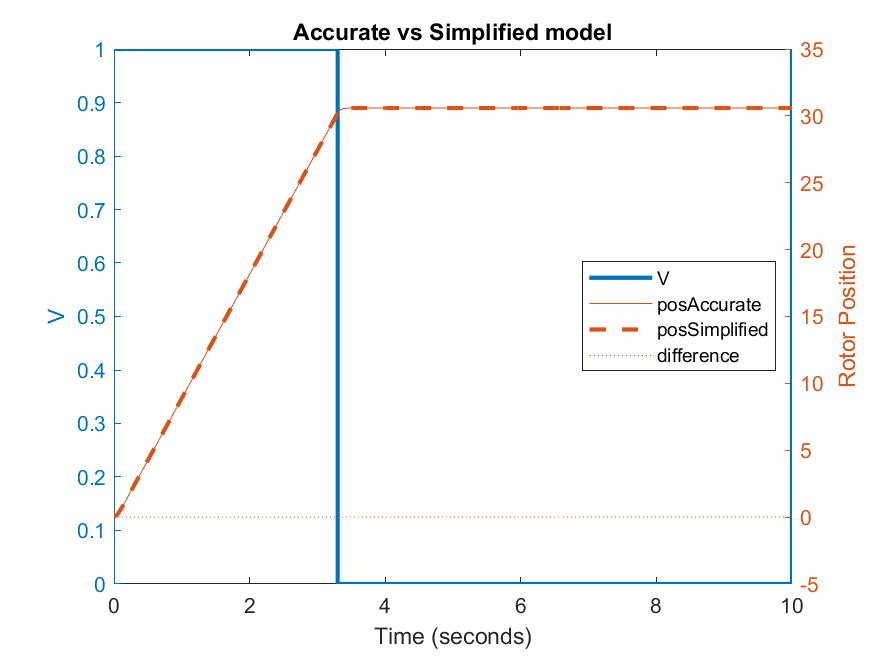
\includegraphics[width=.6\textwidth]{modelAccurateVsSimplified.png}
    \caption{Comparison of accurate and simplified single-link manipulator models}
    \label{fig:modelAccurateVsSimplified}
\end{figure}